\definecolor{gray}{rgb}{0.8,0.8,0.8}
\def\tblhcolor {gray}


\chapter{\CoP\,-- A Survey of Important Results}
\label{ch:copsurvey}

This chapter surveys several results that are significant to this
thesis or to \COP in general. These predominantly pertain to
characterizations of \COP, algorithmic tests to check for \COP (COT),
optimization problems on binary matrices that do not have \COP and
some applications of \COP.

\tnote[important]{ADD: have a few lines about organization of chapter}

\section{\COP in Graph Theory}

\COP is closely connected to several types of graphs by way of
describing certain combinatorial graph properties. There are also
certain graphs, like convex bipartite graphs, that are defined solely
by some of its associated matrix having \COP.  In this section we will
see the relevance of \cop to graphs.  To see this we introduce certain
binary matrices that are used to define graphs in different
ways. While adjacency matrix is perhaps the most commonly used such
matrix, Definition~\ref{def:graphmatrices} defines this and a few
more.

% \begin{definition}{\emph{Matrices that define
%       graphs.\cite[Def.~2.4]{d08phd}}} %
\begin{definition}
  {\em Matrices that define graphs. \cite[Def.~2.4]{d08phd}.}  
  \label{def:graphmatrices} 
  Let $G$ and $H$ be defined as follows. $G = (V,E_G)$ is a graph with
  vertex set $V = \{v_i \mid i \in [n]\}$ and edge set $E_G \subseteq
  \{(v_i,v_j) \mid i, j \in [n]\}$ such that $|E_G| = m$. $H = (A, B,
  E_H)$ is a bipartite graph with partitions $A = \{a_i \mid i \in
  [n_a]\}$ and $B = \{b_i \mid i \in [n_b]\}$.
  \begin{enumerate}[{\ref{def:graphmatrices}}--i.]
  \item \emph{Adjacency matrix} of $G$ is the symmetric $n \times n$
    binary matrix $M$ with $m_{i,j} = \un$ \iff $(v_i,v_j) \in E_G$
    for all $i,j \in [n]$.
  \item \emph{Augmented adjacency matrix} of $G$ is obtained from its
    adjacency matrix by setting all main diagonal elements to \un, \ie
    $m_{i,i} = \un$ for all $i \in [n]$.
  \item \emph{Maximal clique matrix} or \emph{vertex-clique incidence
      matrix} of $G$ is the $n \times k$ binary matrix $M$ with
    $m_{i,j} = \un$ \iff $v_i \in C_j$ for all $i \in [n], j \in [k]$
    where $\{C_j \mid j \in [k]\}$ is the set of maximal cliques of
    $G$.
    \label{def::maxcliquematrix}
  \item \emph{Half adjacency matrix} of $H$ is the $n_a \times n_b$
    binary matrix $M$ with $m_{i,j} = \un$ \iff $(a_i, b_j) \in E_H$.
  \end{enumerate}
\end{definition}

\figgraphmatrices

Now we will see in Definition~\ref{def:graphwithcop} certain graph
classes that is related to \COP or \CROP.\\

\begin{definition}{\emph{Graphs that relate to
      COP.\cite[Def.~2.5]{d08phd}}} %
  \label{def:graphwithcop} %
  Let $G$ be a graph and $H$ be a bipartite graph.

  \begin{enumerate}[\ref{def:graphwithcop}--i.]
  \item $G$ is \emph{convex-round} if its adjacency matrix has the
    \CROP.
  \item \label{def::concave-round} $G$ is \emph{concave-round} if its
    augmented adjacency matrix has \CROP. \tnote{cite BHY00}
    \tnote[minor]{add CROP to glossary}
  \item $G$ is an \emph{interval graph} if its vertices can be mapped
    to intervals on the real line \stt two vertices are adjacent \iff
    their corresponding intervals overlap \tnote{cite Ben59, Haj57}.
    $G$ is an interval graph \iff its maximal clique matrix has COP
    \cite{fg65}\endnote{This follows \cite{gh64} which states that the
      maximal cliques of interval graph $G$ can be linearly ordered
      \stt for all $v \in V(G)$, cliques containing $v$ are
      consecutive in the ordering \cite[Th. 8.1]{mcg04}.}

    \begin{enumerate}[a.]
    \item $G$ is a \emph{unit interval graph} if it is an interval
      graph \stt all intervals have the same length.\endnotemark[2]
    \item $G$ is a \emph{proper interval graph} if it is an interval
      graph \stt no interval properly contains another.\endnote{The
        set of unit interval graphs and the set of proper interval
        graphs are the same} \tnote{cite {rob69,gar07} in endnote. pg
        33 dom}
    \end{enumerate}
 \item $G$ is a \emph{circular-arc graph} if its vertices can be
    mapped to a set of arcs on a circle \stt two vertices are adjacent
    \iff their corresponding arcs overlap.\tnote[pressing]{how is
      CO/ROP related?}
  \item $H$ is \emph{convex bipartite on columns (rows)} if its half
    adjacency matrix has \COP on rows (columns).%
    \label{def::convexbi}
  \item $H$ is \emph{biconvex bipartite} or \emph{doubly
      convex}\cite{yc95} if its half adjacency matrix has \COP on both
    rows and columns.
  \item $H$ is \emph{circular convex} if its half adjacency matrix has
    \CROP.
  \end{enumerate}
\end{definition}

Interval graphs and circular-arc graphs have a long history in
research. The interest around them is due to their very desirable
property that several problems that are NP-hard\tnote[minor]{all NPC
  problems are NPH yes?} on general graphs are not so in these graph
classes, \ie they are polynomial time solvable on them. In a similar
fashion, a lot of problems that are hard on general matrices have
efficient solutions on matrics with \COP or \CROP \cite[more citations
pg.\,33]{d08phd}. 

Table~\ref{tab:graphmatrices} summarises the way these graphs are
characterized by their matrices having \COP or \CROP.
Our focus in this chapter (and thesis) is mainly \COP and 
having seen how useful \COP is in identifying or characterizing many
types of graphs, we will now see results that study recognition of \COP
in matrices in the following section.


\temptext{ tab~\ref{tab:graphmatrices} -  have an abridged version
  of table 2.1 in dom. see notes for the possibility of a
  ``circle diagram''.} 
\begin{table}[htbp]
  \centering
 \caption{\figtabsize Graph matrices \temptext{PLACEHOLDER}}
  \label{tab:graphmatrices}
\end{table}

%\clearpage      % Print pending floats

\section{Matrices with COP}
\label{sec:surveycoptest}

The most important questions with respect to a particular 
property desired in a structure/object are perhaps the following.
\begin{itemize}%[]
\singlespacing
\item Does the desired property exist in the given input?
\item If the test is affirmative, what is a certificate of the affirmative?
\item If the test is negative, what are the optimization possibilities
  for the property in the input? In other words, how close to having the
  property can the input be?
\item If the test is negative, what is a certificate of the negative?
\end{itemize}

In this section and the rest of the chapter we see results that shaped the
correponding areas respectively for \cop in binary matrices.

\begin{enumerate}[a.]
\singlespacing
\item \label{q:testcop} Does a given binary matrix have \COP?
\item \label{q:copperm} What is the \COP permutation for the given matrix with \COP?
\item \label{q:copopt} What are the optimizations possible and practically useful on
  the given matrix without \COP?
\item \label{q:nocopcert} If algorithm for (\ref{q:testcop}) returns
  \textbf{false}, can a certificate for this be computed?
\end{enumerate}

Without doubt, besides computing answers to these questions, we are
interested in the efficiency of these computations in terms of
computational complexity theory. Results towards
questions~(\ref{q:testcop}) and (\ref{q:copperm}) are surveyed in this
section. Those for question~(\ref{q:copopt}) are discussed in
Section~\ref{sec:surveycopopt} and question~(\ref{q:nocopcert}) is discussed
in Section~\ref{sec:surveycertalgo}.

It may be noted that one way to design an algorithm to test for \COP
is by deriving one from any interval graph recognition algorithm using the
result {\sc hmpv00}\tnote{cite hmpv00} \tnote{in endnote put the theorem 2.7 - dom
  pg 43} \cite{d08phd} which demonstrates how such a derivation can be
done. However, this does not necessarily yield an efficient
algorithm. We will see results that directly solve the problem on
matrices since it is known that questions~(\ref{q:testcop}) and
(\ref{q:copperm}) stated above for \COP are efficiently solvable.
Table~\ref{tab:cophistory} gives a snapshot of these results.

\begin{table}[htbp]
  \centering
   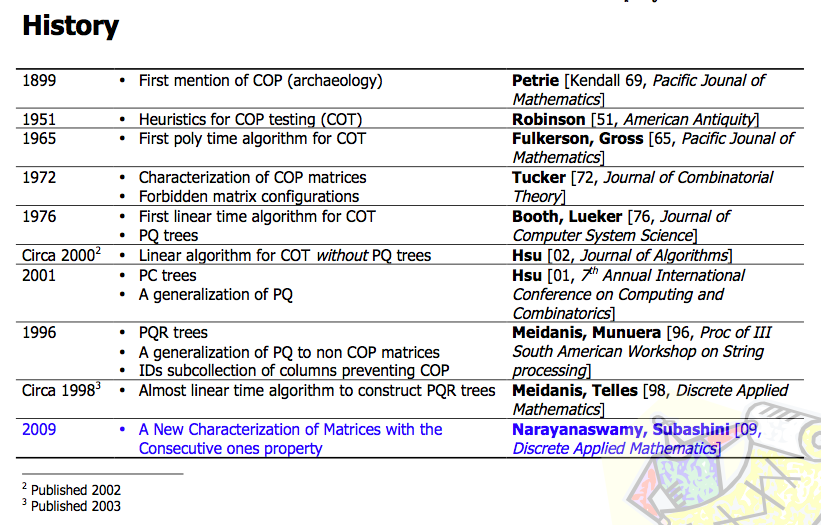
\includegraphics[scale=0.5]{../img/cophistory.png} % TEMPORARY

  \caption[\figtabsize A brief history of \COP research]{\figtabsize A
    brief history of \COP research \temptext{ OLD IMG - PLACEHOLDER - A LATEX
    TABLE WILL REPLACE THIS + WILL BE UPDATED }}
  \label{tab:cophistory}
\end{table}

%\clearpage
\subsection{Tucker's forbidden submatrices for \COP}

% \change{While it is remarkable that the first polynomial time
%   algorithm for \COP testing came in }{The first polynomial time
%   algorithm for \COP testing came in }\cite{fg65} \change{,}{.}
% \change{it is safe to say that the most}{A few years later, a very}
% significant result in understanding \COP came \remove{a few years
%   later} from Tucker which gave a combinatorial (negative)
% characterization of matrices with COP \cite{at72}.
A polynomial time algorithm for \COP testing was seen for the first
time in \cite{fg65} which uses overlapping properties of columns with
\un s. A few years later, a deeply significant result based on very
different ideas in understanding \COP came from Tucker which gave a
combinatorial (negative) characterization of matrices with COP
\cite{at72}. This result influenced most of the \COP results that
followed in the literature \annote[pressing]{including linear time
  algorithms}{did it? which ones?} for \COP recognition.

\cite{at72} discovered certain forbidden structures for convex
bipartite graphs\endnote{The terminology in \cite{at72} differs. It
  uses the term {\em graphs with $V_1$-consecutive arragement} instead
  of {\em convex bipartite graphs}.} and by definition of this graph
class, this translates to a set of forbidden submatrices for matrices
with \cop.  The following are the theorems from \cite{at72} that
acheived this characterization.


Theorem~\ref{th:tuckeratfree} proves that convex bipartite graphs
cannot have {\em asteroidal triples}\endnote{If $G = (V,E)$ is a
  graph, a set of three vertices from $V$ form an {\em asteroidal
    triple} if between any two of them there exists a path in $G$ that
  does not contain any vertex from the closed neighborhood of the
  third vertex.} contained in the corresponding vertex
partition\endnote{The partition corresponds to columns (rows) if its
  half adjacency matrix has \COP columns (rows).}.
Theorem~\ref{th:tuckerforbidden} shows what are the structures in a
bipartite graph that force one of its vertex partitions to have
asteriodal triples -- in other words, it identifies the subgraphs that
prevent the graph from being convex bipartite.


\begin{theorem}
  (\cite[Th.~6]{at72}, \cite[Th.~2.3]{d08phd})\\
  A bipartite graph $G = (V_1, V_2, E)$ is convex bipartite on
  columns\endnote{Abridged to match terminology adopted in this
    document. See previous note.} \iff $V_1$ contains no asteroidal
  triple of $G$.
  \label{th:tuckeratfree}
\end{theorem}

\begin{theorem}
  (\cite[Th.~7]{at72}, \cite[Th.~2.4]{d08phd})\\
  In a bipartite graph $G = (V_1, V_2, E)$ the vertex set $V_1$
  contains no asteroidal triple \iff $G$ contains none of the graphs
  $G_{I_k}$, $G_{II_k}$, $G_{III_k}$ (with $k \ge 1$), $G_{IV}$,
  $G_{V}$ as shown in Figure~\ref{fig:forbiddensubgraphs} as subgraphs.
  \label{th:tuckerforbidden}
\end{theorem}


\begin{figure}[htbp]
  \centering
  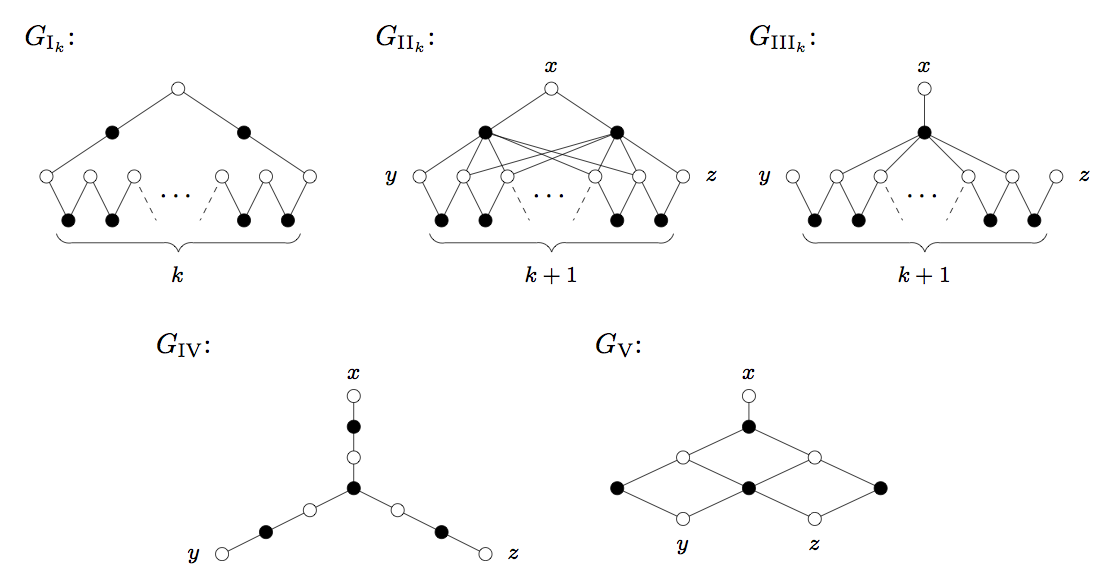
\includegraphics[scale=0.35]{../img/tuckersforbiddensubgraphs.png}  
  \caption[\figtabsize Tucker's forbidden subgraphs]{\figtabsize Tucker's
    forbidden subgraphs for convex bipartite graphs. \temptext{ PLACEHOLDER
    IMG }} 
  \label{fig:forbiddensubgraphs}
\end{figure}

Theorem~\ref{th:tuckeratfree} and Theorem~\ref{th:tuckerforbidden}
result in the following Theorem~\ref{th:tuckercop} which characterizes
matrices with \COP.

\begin{theorem}
  (\cite[Th.~9]{at72}, \cite[Th.~2.5]{d08phd})\\
  A matrix $M$ has \COP \iff it contains none of the matrices 
$M_{I_k}$, $M_{II_k}$, $M_{III_k}$ (with $k \ge 1$), $M_{IV}$,
  $M_{V}$ as shown in Figure~\ref{fig:forbiddensubmatrices} as submatrices.
  \label{th:tuckercop}
\end{theorem}

\begin{figure}[htbp]
  \centering
  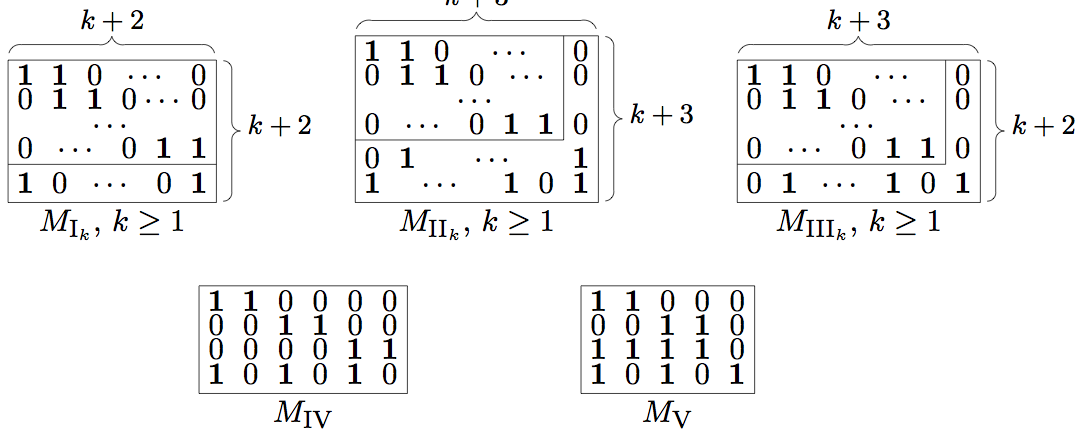
\includegraphics[scale=0.35]{../img/tuckersforbiddensubmatrices.png}  
  \caption[\figtabsize Tucker's forbidden submatrices]{\figtabsize Tucker's
    forbidden submatrices for convex bipartite graphs. \temptext{ PLACEHOLDER
    IMG }} 
  \label{fig:forbiddensubmatrices}
\end{figure}

It can be verified that the matrices in
Figure~\ref{fig:forbiddensubmatrices} are the half adjacency matrices
of the graphs in Figure~\ref{fig:forbiddensubgraphs} respectively
which is not surprising due to
Definition~\ref{def:graphwithcop}~\ref{def::convexbi}.

%\clearpage
\subsection{$PQ$ tree -- a linear COT algorithm}

Booth and Lueker in their paper \cite{bl76} gave the first linear
algorithm for \cop testing by way of an interval graph recognition
algorithm. Their result has close relations to the characterization of
interval graphs by \cite{gh64}. A graph $G$ is an interval graph \iff
all its maximal cliques can be linearly ordered \stt for any vertex
$v$ in $G$, all the cliques that $v$ is incident on are consecutive in
this order. Clearly, this means that the maximal clique incidence
matrix\footnote{
  Definition~\ref{def:graphmatrices}~\ref{def::maxcliquematrix}} must
have \COP on rows. This algorithm constructs a data structure called
\PQtree. A \PQtree represents all the \COP orderings of the matrix it
is associated with. \cite{bl76}'s algorithm uses the fact that if a
matrix has \COP, a \PQtree for it can be constructed. It is
interesting to note that aside from interval graph recognition and
\COP testing, \PQtree is also useful in other applications like
finding planar embeddings of planar graphs \cite{lec67,mcc04} and
recognizing \CROP in a matrix.

\begin{definition}[\emph{\PQtree \cite{bl76, mcc04}}]\\
  A \PQtree of matrix $M$ with \COP, is a tree with the following properties.
  \begin{enumerate}[i.]
    \singlespacing
  \item Each leaf uniquely represents a row (column) of $M$. The leaf
    order of the tree gives a \COP order for column (row)\endnote{Note
      that \COP order for column requires permutation of rows and vice
      versa.} for $M$.
  \item Every non-leaf node in the tree are labeled $P$ or $Q$.
  \item \label{def::nodep} The children of $P$ nodes are
    unordered. They can be permuted in any fashion to obtain a new
    \COP order for $M$.
  \item \label{def::nodeq} The children of $Q$ nodes are linearly
    ordered. Their order can be reversed to get obtain a new \COP
    order for $M$.
  \end{enumerate}
  \label{def:pqtree}
\end{definition}

Thus, effectively, there exists a bijection between set of matrices
with \COP and the set of \PQtrees (accurately speaking, each matrix
with \COP bijectively maps to an equivalence class of \PQtrees due to
properties (\ref{def::nodep}) and (\ref{def::nodeq})). See
Figure~\ref{fig:pqtree} for an example of \PQtree.

\begin{figure}[htbp]
  \centering
  \begin{tabular}[h]{lr}
    \begin{tabular}[h]
      {>{\columncolor{\tblhcolor}} l lllllllllll|}
      \hline
      $r_1$   &\un &0   &\un &0   &0   &0    &0   \\
      $r_2$   &\un &0   &\un &0   &0   &0    &0   \\
      $r_3$   &\un &0   &0   &\un &0   &0    &0   \\
      $r_4$   &\un &0   &0   &\un &0   &0    &0   \\
      $r_5$   &\un &0   &0   &0   &0   &0    &0   \\
      $r_6$   &\un &\un &0   &0   &0   &0    &0   \\
      $r_7$   &0   &\un &0   &0   &0   &\un  &0   \\
      $r_8$   &0   &\un &0   &0   &\un &\un  &0   \\
      $r_9$   &0   &\un &0   &0   &\un &\un  &0   \\
      $r_{10}$ &0   &\un &0   &0   &\un &\un  &\un \\
      $r_{11}$ &0   &\un &0   &0   &\un &0    &\un \\
      \hline
    \end{tabular}
    &
    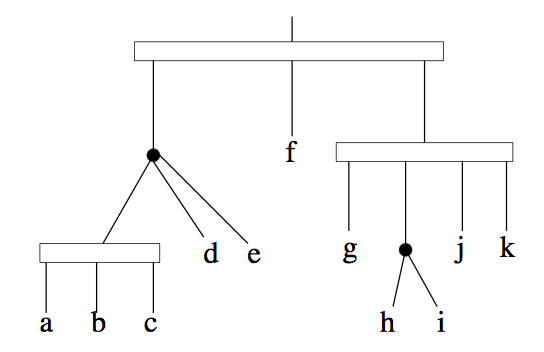
\includegraphics[scale=0.3]{../img/pqtree.png}
    
  \end{tabular}
 
  \caption[\figtabsize An example for \PQtree]{\figtabsize An example for \PQtree.
    Permuting the order of the left child of the root, we see that
    \temptext{(d,a,b,c,e,f,g,h,i,j,k)} is a \COP order. Reversing the
    order of the right child of the root, we see that
    \temptext{(a,b,c,d,e,f,k,j,h,i,g) } is yet another \COP order. \temptext{PLACEHOLDER IMG.}
    \cite[Fig.~1\endnote{\cite{mcc04}illustrates \COP on rows. Our
      convention in this document is \COP on columns and thus example
      matrix has been transposed. }]{mcc04}}
  \label{fig:pqtree}
\end{figure}

The \cite{bl76} algorithm with input $n \times m$ matrix $M$ starts
with a \PQtree for a vacuous $n \times 0$ matrix $M'$ (submatrix
induced by 0 columns). This is known as a {\em universal} \PQtree
which is one with its root as a $P$ node and only leaves as its
children -- each leaf representative of a row of input (by definition
of \COP for columns). This induced submatrix $M'$ vacuously has \COP.
Each column is then added iteratively to $M'$ to check if the new $M'$
has \COP.  By a complicated, but linear, procedure the algorithm does
one of the following actions in each iteration: (a) declare that $M$
has no \COP, or (b) modify the current \PQtree to represent the new
$M'$ (which clearly, must have \COP, since if not, option (a) would
have been executed).

After the invention of \PQtrees, there has been several variants of
the same with either simpler procedure of construction, like \PCtree
\cite{wlh01}\endnote{First appeared in
  \cite{wlh92_isaac}.\tnote{check}} or a generalization of it, like
generalized \PQtree \cite{mcc04}. \PQRtree is another generalization
of \PQtree by \cite{mm96,mpt98}. There algorithm was improved by
\cite{tm05} \tnote{improved in terms of
  what?}. % describes an improved algorithm to
% build PQR trees.
    
\temptext{Expand a little more on PC trees and PQR trees.}

We will see more of \PQRtree in Section~\ref{sec:surveycertalgo}


\temptext{
  \begin{enumerate}[ -I-]
  \item  Variations - PQR, PC etc. [MM96, Hsu01, McC04]\\
    Generalized PQ trees McC04 - brief. Will be elaborated in
    Section~\ref{sec:surveycertalgo}\\
    Hsu also invented PC trees \cite{wlh01}\tnote{This result first
      appeared inproc ISAAC92} which is claimed to be much easier to
    implement.
  \item Set theoretic characterizations [Hsu02, NS09]\\
    \cite{wlh02} describes the simpler algorithm for
    COT.\tnote[pressing]{in terms of what?}\\
    \cite{nsnrs09} describes a characterization of consecutive-ones
    property solely based on the cardinality properties of the set
    representations of the columns (rows); every column (row) is
    equivalent to a set that has the row (column) indices of the rows
    (columns) that have one entries in this column (row). This is
    interesting and relevant, especially to this thesis because it
    simplifies COT to a great degree by reducing the solution search
    space owing to the a simple set theoretic characterization.\\
  \item Parallel algorithms [AS95, BS03, CY91]
  \end{enumerate}

}


\tnote[pressing]{ The results in cite~{bl76} on COT are based on the
   result that interval graphs are AT-free chordal graphs.
 -  Tucker's?}%


\tnote[pressing]{cite~{fg65} uses these results to give the first polynomial
  time algorithm for COT. WHICH RESULTS? \ \ \ \ \ check. how do they use it?}%


\tnote[pressing]{ADD: peo exists iff chordal. lexicographic BFS
  [tag:chordalGraph]} %


%\clearpage      % Print pending floats
\section{Optimization problems in COP}
\label{sec:surveycopopt}
\tnote{Expand on ref:sec:optcop}

%{\color{blue} \footnotesize
\temptext{
So far we have been concerned about matrices that have the consecutive
ones property. However in real life applications, it is rare that data
sets represented by binary matrices have COP, primarily due to the
noisy nature of data available. At the same time, COP is not arbitrary
and is a desirable property in practical data representation
\cite{co98,jkckv04,k77}. In this context, there are several
interesting problems when a matrix does not have COP but is ``close''
to having COP or is allowed to be altered to have COP. These are the
optimization problems related to a matrix which does not have
COP. Some of the significant problems are surveyed in this section.

\tnote{ -- sect 4.1 in cite:d08phd has many results
  surveyed. hardness results, approx. results. results are usually for
  a class of matrices $(a,b)$ where number {\un}s in columns and rows
  are restriced to $a$ and $b$ . -- problem of flipping at most $k$
  entries of $M$ to make it attain COP. this is NP complete
  cite:b75-phd}\tnote{(1) scite:lb62 showed that interval graphs
  are AT-free.  describe AT (2) show the close relationship b/w COP
  and graphs sec 2.2, pg 31} \cite{at72} showed that a matrix that
does not have COP have certain substructures that prevent it from
having COP. Tucker classified these forbidden substructures into five
classes of submatrices. This result is presented in the context of
convex bipartite graphs which \cite{at72} proved to be
AT-free\tnote{ check this up. give details. - doms'}. By
definition, convex bipartite graph have half adjacency matrices that
have COP on either rows or columns (graph is biconvex if it has COP on
both)\cite{d08phd}. A half adjacency matrix is a binary matrix
representing a bipartite graph as follows. The set of rows and the set
of columns form the two partitions of the graph. Each row node is
adjacent to those nodes that represent the columns that have {\un}s in
the corresponding row. \cite{at72} proves that this bipartite graph
has no asteroidal triple if and only if the matrix has COP and goes on
to identify the forbidden substructures for these bipartite
graphs. The matrices corresponding to these substructures are the
forbidden submatrices.

Once a matrix has been detected to not have COP (using any of the COT
algorithms mentioned earlier), it is naturally of interest to find out
the smallest forbidden substructure (in terms of number of rows and/or
columns and/or number of entries that are {\un}s). \cite{d08phd}
discusses a couple of algorithms which are efficient if the number of
{\un}s in a row is small. This is of significance in the case of
sparse matrices where this number is much lesser than the number of
columns. $(*,\Delta)${\em -matrices} are matrices with no restriction
on number of {\un}s in any column but has at most $\Delta$ {\un}s in
any row. {\sc Min COS-R (Min COS-C), Max COS-R (Max COS-C)} are
similar problems which deals with inducing COP on a matrix. In {\sc
  Min COS-R (Min COS-C)} the question is to find the minimum number of
rows (columns) that must be deleted to result in a matrix with COP.
In the dual problem {\sc Max COS-R (Max COS-C)} the search is for the
maximum number of rows (columns) that induces a submatrix with
COP. Given a matrix $M$ with no COP, \cite{b75-phd} shows that finding
a submatrix $M'$ with all columns\tnote{check if b75 deals with
  COP col or COP row. also is it any submatrix with k less than r rows
  or submatrix must have all columns?} but a maximum cardinality
subset of rows such that $M'$ has COP is NP complete. \cite{hg02}
corrects an error of the abridged proof of this reduction as given in
\cite{gj79}.  \cite{d08phd} discusses all these problems in detail
giving an extensive survey of the previously existing results which
are almost exhaustively all approximation results and hardness
results. Taking this further, \cite{d08phd} presents new results in
the area of parameterized algorithms for this
problem\tnote{elaborate - what are the results?}.

Another problem is to find the minimum number of entries in the matrix
that can be toggled to result in a matrix with COP.  \cite{v85}
discusses approximation of {\sc COP Augmentation} which is the problem
of changing of the minimum number of zero entries to {\un}s so that
the resulting matrix has COP. As mentioned earlier, this problem is
known to be NP complete due to \cite{b75-phd}. \cite{v85} also proves,
using a reduction to the longest path problem, \tnote{or is it a
  survey of another result?  check.} that finding a Tucker's forbidden
submatrix of at least $k$ rows is NP complete. \tnote{how is this
  different from booth's 75 result??}  \tnote{where should this go?
  cite|tz04 (approx submatrix with COP sparse matrices)}

\cite{jkckv04} discusses the use of matrices with almost-COP (instead
of one block of consecutive {\un}s, they have $x$ blocks, or {\em
  runs}, of consecutive {\un}s and $x$ is not too large) in the
storage of very large databases.  The problem is that of reordering of
a binary matrix such that the resulting matrix has at most $k$ runs of
{\un}s. This is proved to be NP hard using a reduction from the
Hamiltonian path problem.\tnote{Theorem 2.1 in jkckv} \tnote{(1) A
  connection of COP problem to the travelling salesman problem is also
  introduced. what does this mean? -- COP can be used as a tool to
  reorder $0.5T \le runs(M) \le T$. (2) The optimization version of
  the $k$-run problem, i.e. minimization of number of blocks of ones
  is proven to be NP complete by cite:k77}\tnote{are these two the
  same?} \tnote{what is the reduction?} \tnote{other problems similar
  to COP -- cite:ckl96 (ILP, circ ones, one drop) -- cite:th98
  (generalization of COP - minimax, biotonic column) Tucker} 


}

\section{Certifying Algorithms}
\label{sec:surveycertalgo}
%\tnote{Expand on sec:appcertalgo} \tnote{ (certification McC04
%theme)}

\temptext{ Certifying algorithm (Generalized PQ trees) [McC04] -- Move this to section on
    certifying algo. 

\cite{mcc04} describes a different approach to COT. While all previous
COT algorithms gave the COP order if the matrix has the property but
exited stating negative if otherwise, this algorithm gives an evidence
by way of a certificate of matrix even when it has no COP. This
enables a user to verify the algorithm's result even when the answer
is negative. This is significant from an implementation perspective
because automated program verification is hard and manual verification
is more viable. Hence having a certificate reinforces an
implementation's credibility. Note that when the matrix {\em has} COP,
the COP order is the certificate.  The internal machinery of this
algorithm is related to the weighted betweenness problem
addressed\tnote{in what way??} in \cite{co98}.  \tnote{expand
  on the COP order graph creation and it having to be bipartite for M
  to have COP. and thus an odd cycle being an evidence of no COP.}

}


\section{COP in Relational Database Model}
\label{sec:surveyrdbm}
\tnote{Expand on sec:apprdbm} \tnote{(set systems theme)}

\section{COP in Graph Isomorphism}
\label{sec:surveygraphiso}
\tnote{Expand on sec:appgraphiso} \tnote{(canonization theme)}

\temptext{
The survey from kklv10 conclusion.
}

% \section{Other applications}
% {\tt If any. \tnote{ where should this go?}: (1) cite|jlm97 (application of PQ
%   trees in graphics). (2) helly's theorem citation
%   19XXdgk-Hellystheorem-Danzer-Gruenbaum-Klee}}




\theendnotes\tnote{remove if none.} 




%%%%%%%%%%%%% listing package for pretty formatting BEGIN
% \lstloadlanguages{C}
% \lstset{language=C, commentstyle=\scriptsize,
%   numberstyle=\tiny, numbers=left,               % Line numbers
%   stepnumber=2,numbersep=5pt,firstnumber=10, 
%   showstringspaces=false,                    % No explicit spaces
%   emph={printf},emphstyle=\underbar,      % Specific formatting
%   emph=[2]{sum},emphstyle=[2]\color{blue},      % Sp format (multiple)
%   emph=[3]{i},emphstyle=[3]\color{red}      % Sp format (multiple)
%   } 

%   \begin{singlespacing}
%     % Text inside "lstlisting" env is verbatim.
%     \begin{lstlisting}[keywordstyle=\textbf]      
% int sum;
% int i; /* for loop variable */ 
% sum = 0; 
% for (i=0, i<n; i++) { 
%   sum += a[i]; 
% } 
% printf{"This is stupid."}
%     \end{lstlisting}
%   \end{singlespacing}

%%%%%%%%%%%%% listing package for pretty formatting END

